\documentclass{article}

\usepackage{graphicx}
\usepackage{subcaption}
\usepackage{amssymb}
\usepackage[utf8]{inputenc}
\usepackage[T1]{fontenc}

\renewcommand{\familydefault}{\sfdefault}
\usepackage[scaled=1]{helvet}
\usepackage[helvet]{sfmath}
\everymath={\sf}

\title{Reporte de Evaluación 1}

\author{Diego Iván Moreno Campa}

\date{8 de Marzo, 2018}

\begin{document}

\maketitle

\bigskip

\section{Introducción}

Esta actividad es la primera evaluación de la materia de Física computacional I en la licenciatura de Física.

El propósito de esta actividad es realizar el análisis de unos datos tomados para el nivel del mar y la salinidad en un manglar conocido como El sargento.

\section{Procedimiento}

Comenzamos descargando dos archivos \textit{sargento-270218.csv} para las lecturas del nivel del mar y \textit{sargento-salinidad-270218.csv} para obtener las lecturas de salinidad.

El archivo sargento-270218.csv contiene una tabla con los datos del tiempo, presión absoluta, temperatura en grados centigrados y el nivel del agua en metros. Las mediciones fueron tomadas cada 15 minutos durante el tramo del mes de febrero de 2018.

El archivo sargento-salinidad-270218.csv contiene de manera similar, una tabla con datos del tiempo, "Cond high RNG", temperatura, conductividad específica y por supuesto, salinidad en partes por mil (ppt)

Se limpiaron los archivos utilizando el comando egrep para seleccionar todo renglón que no tuviera la primera y ultima fecha, después con emacs se eliminaron los caractéres que se repetían al utilizar egrep.

Con esto, continuamos a utilizar Python para analizar los datos, utilizando mayormente lo que ya conociamos por las prácticas pasadas.

\subsection{boxplot:}

Después de acomodar los tipos de fecha de cada dataframe, se nos pide realizar gráficas de caja para lo siguiente.
De la misma manera que la actividad 5, se utilizó la gráfica de cajas proporcionada por la librería Seaborn con el siguiente segmento de código, ajustandolo a nuestras necesidades:
\begin{verbatim}
ax = sns.boxplot(x="month", y="CAPE", data=df00)
plt.show()
\end{verbatim}

\begin{itemize}
\item Nivel de mar (metros):
\begin{figure}[h!]
\centering
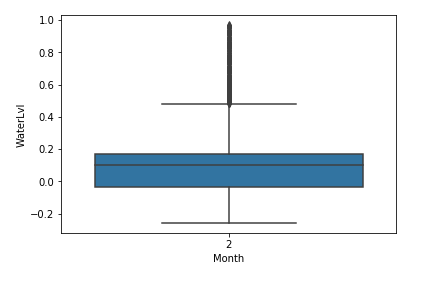
\includegraphics[width=0.4\linewidth]{wtrlvl.png}
\end{figure}

\item Salinidad (ppt):
\begin{figure}[h!]
\centering
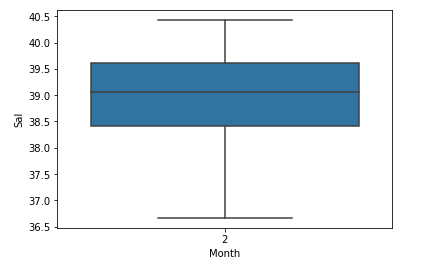
\includegraphics[width=0.4\linewidth]{sal.png}
\end{figure}

\item Temperatura del agua($^\circ$C)
\begin{figure}[h!]
	\begin{subfigure}[b]{0.5\linewidth}
    \raggedleft
	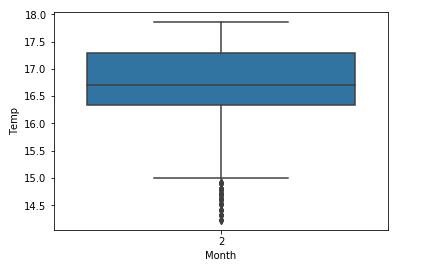
\includegraphics[width=\linewidth]{temp1st.png}
    \caption{Primer Sensor}
	\end{subfigure}
	\begin{subfigure}[b]{0.5\linewidth}
    \raggedright
	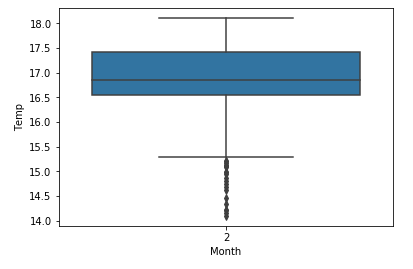
\includegraphics[width=\linewidth]{temp2nd.png}
	\caption{Segundo Sensor}
    \end{subfigure}
\end{figure}

\end{itemize}

\subsection{correlación de Pearson (Regresión líneal):}

Luego, se pide observar las relaciones entre las siguientes variables.
Al igual que en la actividad 5, se utilizó el siguiente código para realizar la regresión lineal, reemplazando "CAPE" y "PW" por lo que deseamos comparar:
\begin{verbatim}
sns.set(style="darkgrid", color_codes=True)

g = sns.jointplot("CAPE", "PW", data=df00, kind="reg",
                   color="r", size=7)
plt.show(g)
\end{verbatim}

\begin{itemize}
\item Nivel de mar-Salinidad:
Para esta gráfica se necesitó juntar las columnas requeridas de cada dataframe, para esto se utilizó \textit{pd.concat}
\begin{figure}[ht!]
\centering
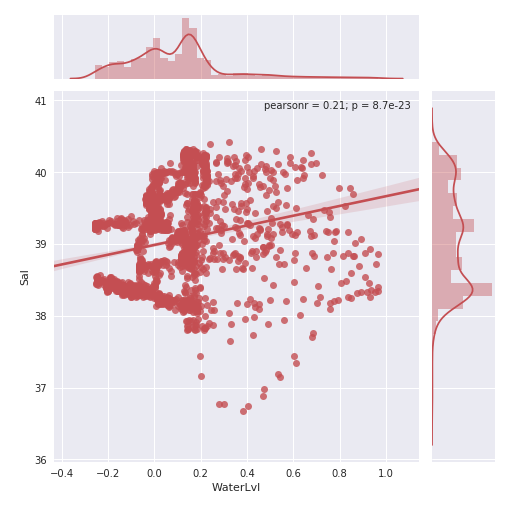
\includegraphics[width=0.4\linewidth]{nivel-salinidad.png}
\end{figure}

\item Nivel de mar-Temperatura del agua:
\begin{figure}[ht!]
\centering
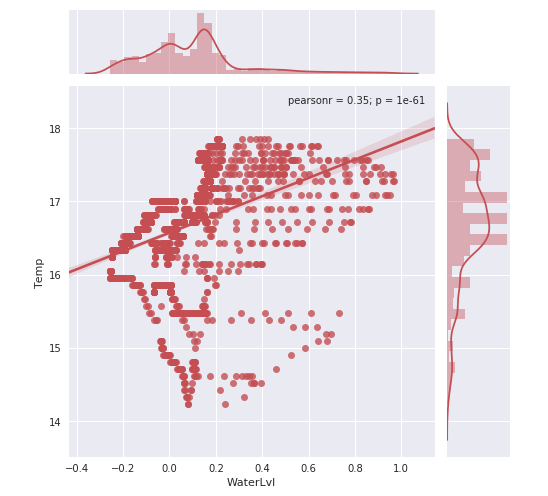
\includegraphics[width=0.4\linewidth]{nivel-temp.png}
\end{figure}

\item Salinidad-Temperatura del agua:
\begin{figure}[ht!]
\centering
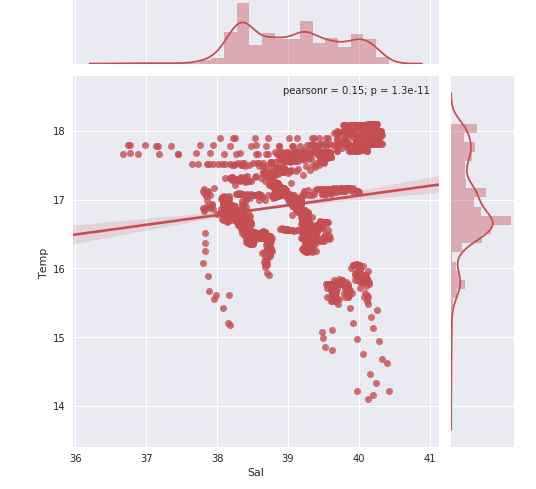
\includegraphics[width=0.4\linewidth]{sal-temp.png}
\end{figure}

\end{itemize}

\subsection{Gráficas independientes:}

Después se procedio a realizar gráficas contra el tiempo utilizando matplotlib de los siguientes datos.
Para realizar estas gráficas se utilizó el segmento de código que utilizamos en la Actividad 2 para graficar los datos individualmente, con su cantidad de mediciones:
\begin{verbatim}
plt.figure(); df.VELS.plot(); plt.legend(loc='best')
plt.title("Variación de la Rapidez de los Vientos")
plt.ylabel("Rapidez (m/s)")
plt.grid(True)
plt.show()
\end{verbatim}

\begin{itemize}
\item Nivel del mar:
\begin{figure}[ht!]
\centering
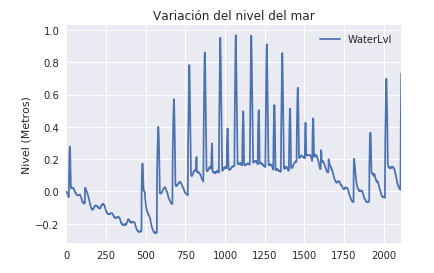
\includegraphics[width=0.4\linewidth]{nivel-tiempo.png}
\end{figure}

\item Salinidad:
\begin{figure}[h!]
\centering
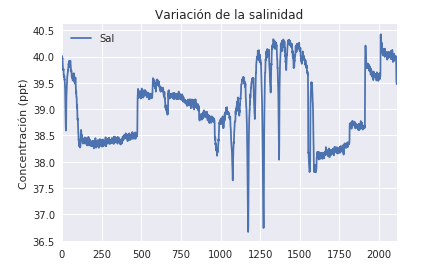
\includegraphics[width=0.4\linewidth]{sal-tiempo.png}
\end{figure}

\item Temperatura:
\begin{figure}[ht!]
\centering
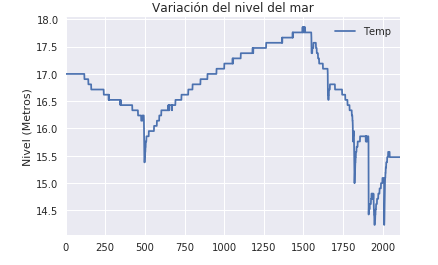
\includegraphics[width=0.4\linewidth]{temp-tiempo.png}
\end{figure}

\end{itemize}

\newpage

\subsection{Gráficas superpuestas con doble eje vertical}

Luego se nos pidió realizar gráficas superpuestas con doble eje vertical utilizando las siguientes variables.
Para este caso se utilizo el siguiente segmento de código para poner dos variables en el eje-y, reemplazando la \textit{x} por nuestro valor ordenado y reemplazando \textit{y1} y \textit{y2} con sus respectivas variables que deseamos comparar:
\begin{verbatim}
fig = plt.figure()
ax1 = fig.add_subplot(111)
ax1.plot(x, y1)
ax1.set_ylabel('y1')

ax2 = ax1.twinx()
ax2.plot(x, y2, 'r-')
ax2.set_ylabel('y2', color='r')
for tl in ax2.get_yticklabels():
	tl.set_color('r')
plt.show()
\end{verbatim}

\begin{itemize}
\item Nivel de mar y Salinidad:
\begin{figure}[h!]
\centering
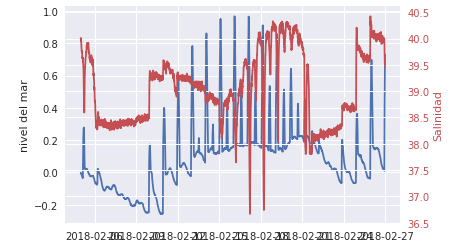
\includegraphics[width=0.4\linewidth]{nivel-sal-tiempo.png}
\end{figure}

\item Nivel de mar y Temperatura:
\begin{figure}[ht!]
\centering
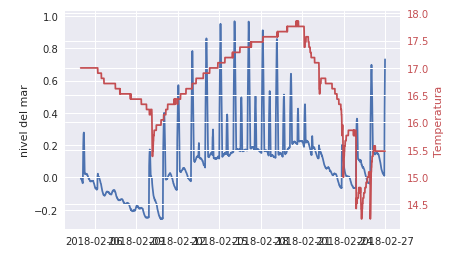
\includegraphics[width=0.4\linewidth]{nivel-temp-tiempo.png}
\end{figure}

\end{itemize}

\newpage

\subsection{Doble eje-y en un intervalo:}

Luego se nos pide revisar si hay alguna relación entre las variables anteriores, para esto veremos un segmento de 5 días en las gráficas anteriores:
Para esto utilizamos el segmento de código anterior para realizar las gráficas, únicamente se agrego la siguiente instrucción para delimitar a la fecha entre los días 10 de febrero y 15 de febrero
\begin{verbatim}
plt.xlim("2018-02-10 00:00:00","2018-02-15 23:00:00")
\end{verbatim}

\begin{itemize}
\item Salinidad y Nivel de mar del 10 de febrero al 15 de febrero:
\begin{figure}[h!]
\centering
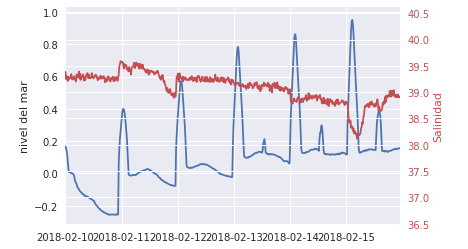
\includegraphics[width=0.4\linewidth]{nivel-sal-5dias.png}
\end{figure}
Considero que no se nota tan claramente una dependencia en este caso, debido a que se mantiene relativamente constante.

\item Nivel de Mar y Temperatura del agua:
\begin{figure}[h!]
\centering
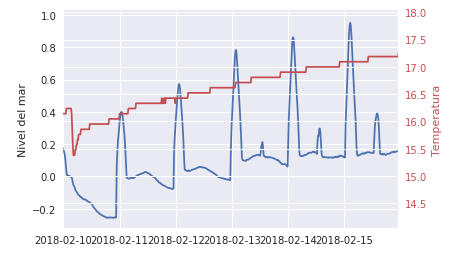
\includegraphics[width=0.4\linewidth]{nivel-temp-5dias.png}
\end{figure}
En este caso parece ser que la temperatura crece junto con el nivel del mar, lo cual da una señal de que haya una dependencia.

\end{itemize}

\end{document}
